% Evidence: results/reviews/2026-10-23/baseline_native_complete/summary.json
\begin{frame}{A matched polymer cycle separates thermal and site effects}
\centering
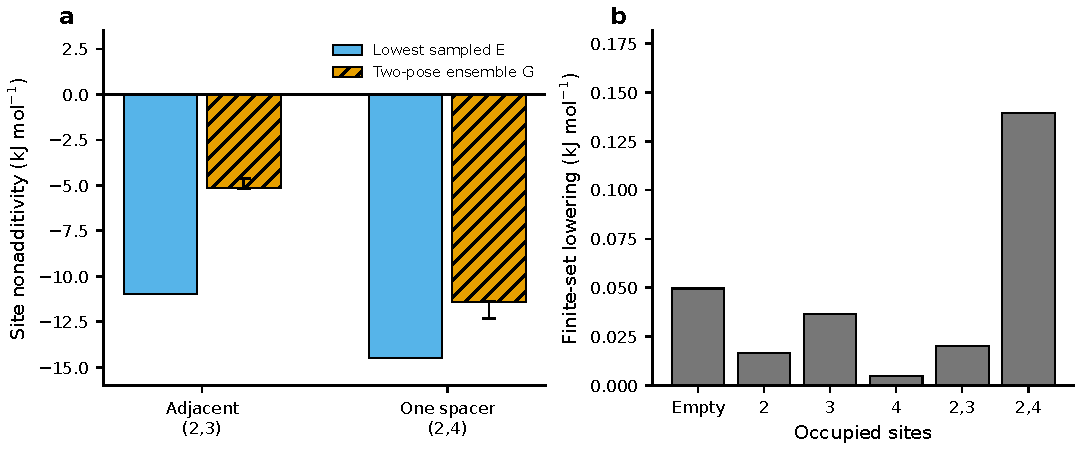
\includegraphics[width=.96\linewidth,height=.66\textheight,keepaspectratio]{../results/figures/polymer_models/conditional_ensemble_baseline.pdf}
\par\smallskip\small
Twelve checked native G values; two poses per graph. Adjacent/one-spacer nonadditivity: $-5.17/-11.39$ kJ/mol.
\par\footnotesize Phthalimide control, one backbone configuration. Whiskers: prescribed rotor-cutoff sensitivity. Broader conformer convergence remains open; no pure motif-binding or electron-transfer-rate claim.
\end{frame}
\begin{frame}{Route thermodynamics still needs quantitative validation}
\begin{block}{A defined term exposes model sensitivity}
For DBU + HCl $\rightarrow$ DBUH$^+$ + Cl$^-$ in MeCN:
\begin{center}
\begin{tabular}{lr}
\toprule
Capture model & $\Delta G$ (kJ/mol)\\
\midrule
Computed separated ions & $-102.78$\\
Author-tabulated pKa anchors at 298.15 K & $-79.97$\\
Difference & $-22.81$\\
\bottomrule
\end{tabular}
\end{center}
\end{block}
\small Exact source temperature/activity conventions remain under review. HCl cancels from the full all-DFT grafting cycle; changing only this term changes shared-error cancellation.
\par\medskip\textcolor{teal}{\textbf{Both BQ signs survive the limited DBU term sensitivity. Full grafting accuracy remains unvalidated.}}
\par\vfill\scriptsize Sources: Leito-group tables; DOI 10.1002/ejoc.201900956 and 10.1002/poc.2946. No exact DIPEA anchor substituted.
\end{frame}
